\subsection{Data analysis}
\label{subsec:ir:data-analysis}

This section will discuss the data processing, including calibration, normalization, and averaging process of the obtained spectra from the FELion instrument combined with FELIX. During the PhD work, an analysis software package called FELionGUI, based on Python 3 was developed \footnote{Vist \url{https://felion-docs.vercel.app/} for FELionGUI documentation}.\\

\begin{figure}[!htb]
    \centering
    
    \begin{subfigure}[b]{0.45\textwidth}
        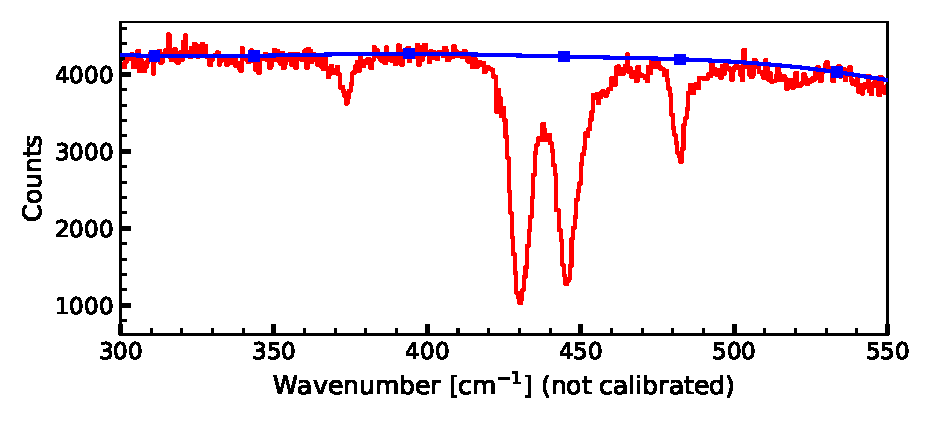
\includegraphics[width=1\textwidth]{figures/IR-data-norm/baseline_correction.pdf}
        \caption{}
        \label{fig:data-process:raw}
    \end{subfigure}
    \hfill
    \begin{subfigure}[b]{0.45\textwidth}
        \centering
        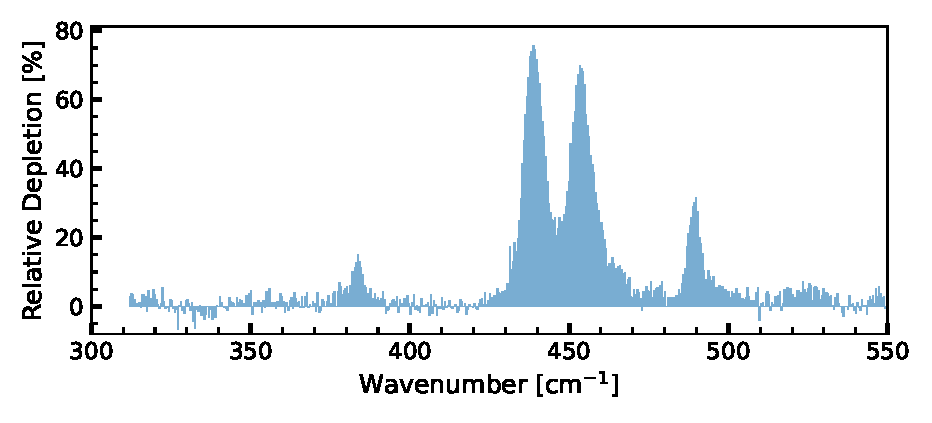
\includegraphics[width=1\textwidth]{figures/IR-data-norm/processed.pdf}
        \caption{}
        \label{fig:data-process:processed}
        \end{subfigure}
    \hfill
    % \begin{subfigure}[b]{0.45\textwidth}
    %     \centering
    %     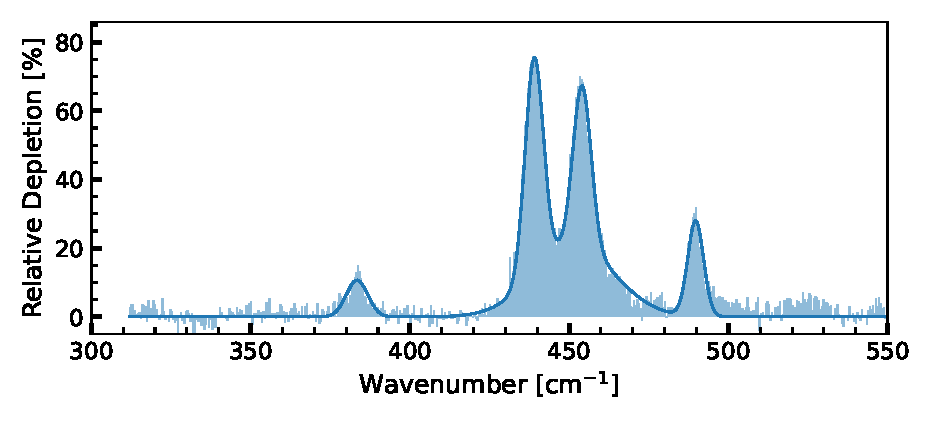
\includegraphics[width=1\textwidth]{figures/IR-data-norm/fitted.pdf}
    %     \caption{}
    %     \label{fig:data-process:fitted}
    %     \end{subfigure}
    % \hfill
    \begin{subfigure}[b]{0.45\textwidth}
        \centering
        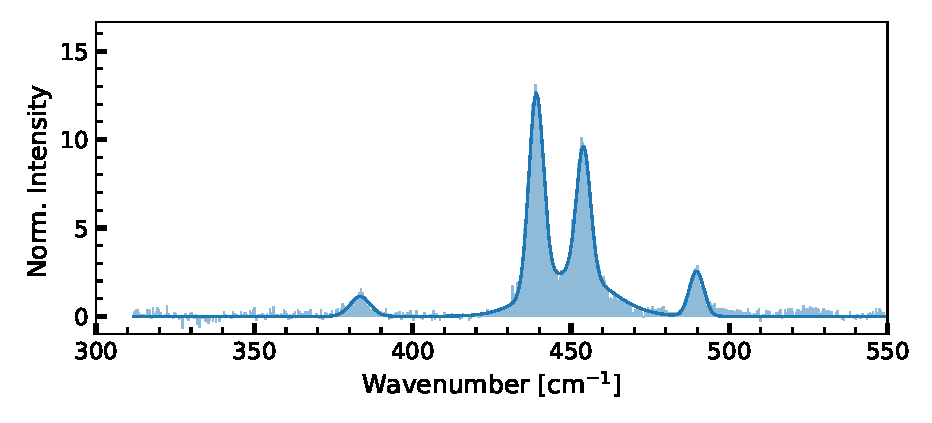
\includegraphics[width=1\textwidth]{figures/IR-data-norm/normalised.pdf}
        \caption{}
        \label{fig:data-process:normalised}
    \end{subfigure}
    
    \caption{Data processing (for Ne-HC$_3$N$^+$ IRPD spectrum using FELIX): (a) is the raw data obtained by directly measuring the depletion counts of formed complex ions in IRPD schemes at varying frequencies. The blue line corresponds to a possible baseline to account for ion count fluctuation. (b) is the first processed spectrum with baseline correction from (a). (c) is the final normalised spectrum (see text) and the solid line corresponds to fitting the spectrum with a multi-component Gaussian function.}
    \label{fig:data-process}
\end{figure}

\textbf{Baseline correction:} The formed ion complex is monitored and counted in the IRPD experiments reported in this thesis. Figure \ref{fig:data-process:raw} shows the measured raw data. Each data point is typically an average of 4 iterations. This spectrum should be baseline corrected for ion count fluctuation. Since even slight changes in the experimental condition, such as temperature, number density, and change in tagging efficiency due to laser heating, etc., can induce a non-linear shift in an otherwise constant background signal. As shown in Figure \ref{fig:data-process:raw}, the solid blue line is the constructed baseline via a cubic spline interpolation and can be manually adjusted. In addition to baseline correction, the raw spectrum needs to be frequency calibrated against the actual frequency output from the radiation source, i.e., using a grating spectrum analyser (FELIX) and manual wavenumber corrections based on a wavemeter (HighFinesse WS - Series) reading (OPO/A system).\\

\textbf{Normalisation and fitting:} Initially, baseline corrected data is a relative depletion ($D$) of complex ions and is given by:

\[ D= 1 - \frac{N_{ON}(\nu)}{N_{OFF}} \] 

where $N_{OFF}$ is the baseline value and $N_{ON}(\nu)$ is the depleted value of the number of complex ions that are observed upon resonant vibrational excitation as shown in Figure \ref{fig:data-process:processed}.

To account for variations of the laser pulse energy $E$, pulse number $n$, and for saturation effects, the signal is normalised ($I$) as given below: 

\[ I [\text{per J}]=\frac{- ln(N_{ON}(\nu)/N_{OFF})}{n \cdot E[\text{in J}]} \]

where $I$ is the intensity in units of relative cross-section per Joule. 

One can obtain a relative cross-section per photon by multiplying $I$ with the wavenumber. Figure \ref{fig:data-process:normalised} shows the final normalised spectrum. The measurements are repeated in the same frequency range for averaging, i.e., the final spectrum is obtained by averaging using statistical binning with a typical bin size of 1.5-2 \wn\ of all normalised data. Line parameters such as band positions, intensities, and line widths (fwhm) are then obtained with statistical errors by fitting a multi-component Gaussian function to the experimental data. 
